\begin{figure}[t!]
    \centering
    \hspace{-12px}
    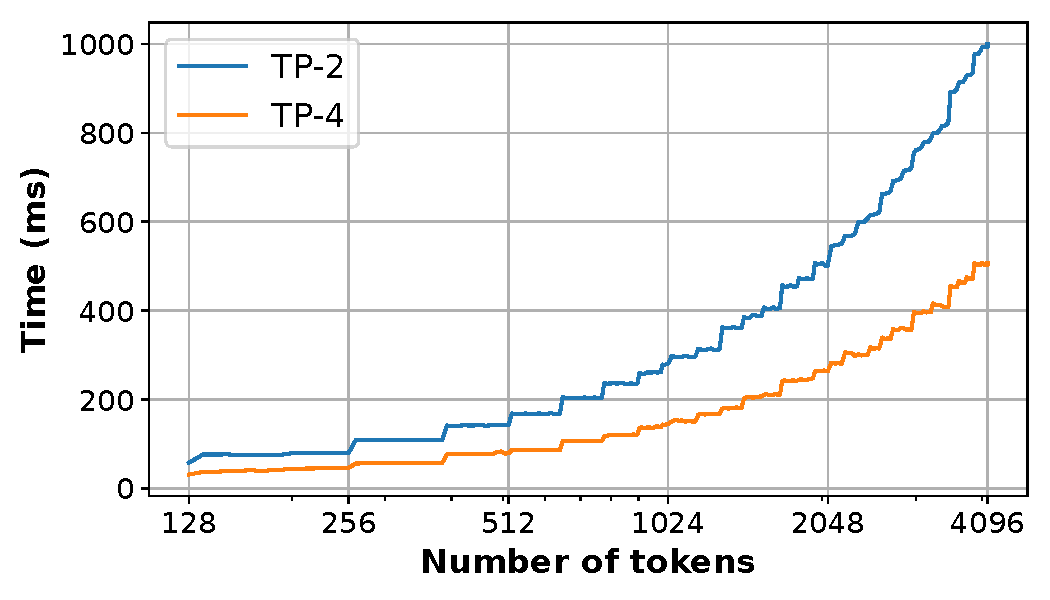
\includegraphics[width=0.45\textwidth]{figures/mlp_num_tokens_vs_time.pdf}
    \caption{Linear layer execution time as function of number of tokens in a batch for \llamaL on A100(s) with different tensor parallel degrees. When the number of tokens is small, execution time is dictated by the cost of fetching weights from HBM memory. Hence, execution time is largely stagnant in the 128-512 tokens range, especially for higher tensor parallel degrees. Once the number of tokens in the batch cross a critical threshold, the operation become compute bound and the runtime increases linearly with number of tokens.}%
    \label{fig:motivation:mlp-time} 
\end{figure}
